% !TEX root = ../main.tex
\chapter{Figures} \label{app:figures}
\begin{figure}[H]
    \centering
    % First row
    \begin{subfigure}[b]{0.48\textwidth}
        \centering
        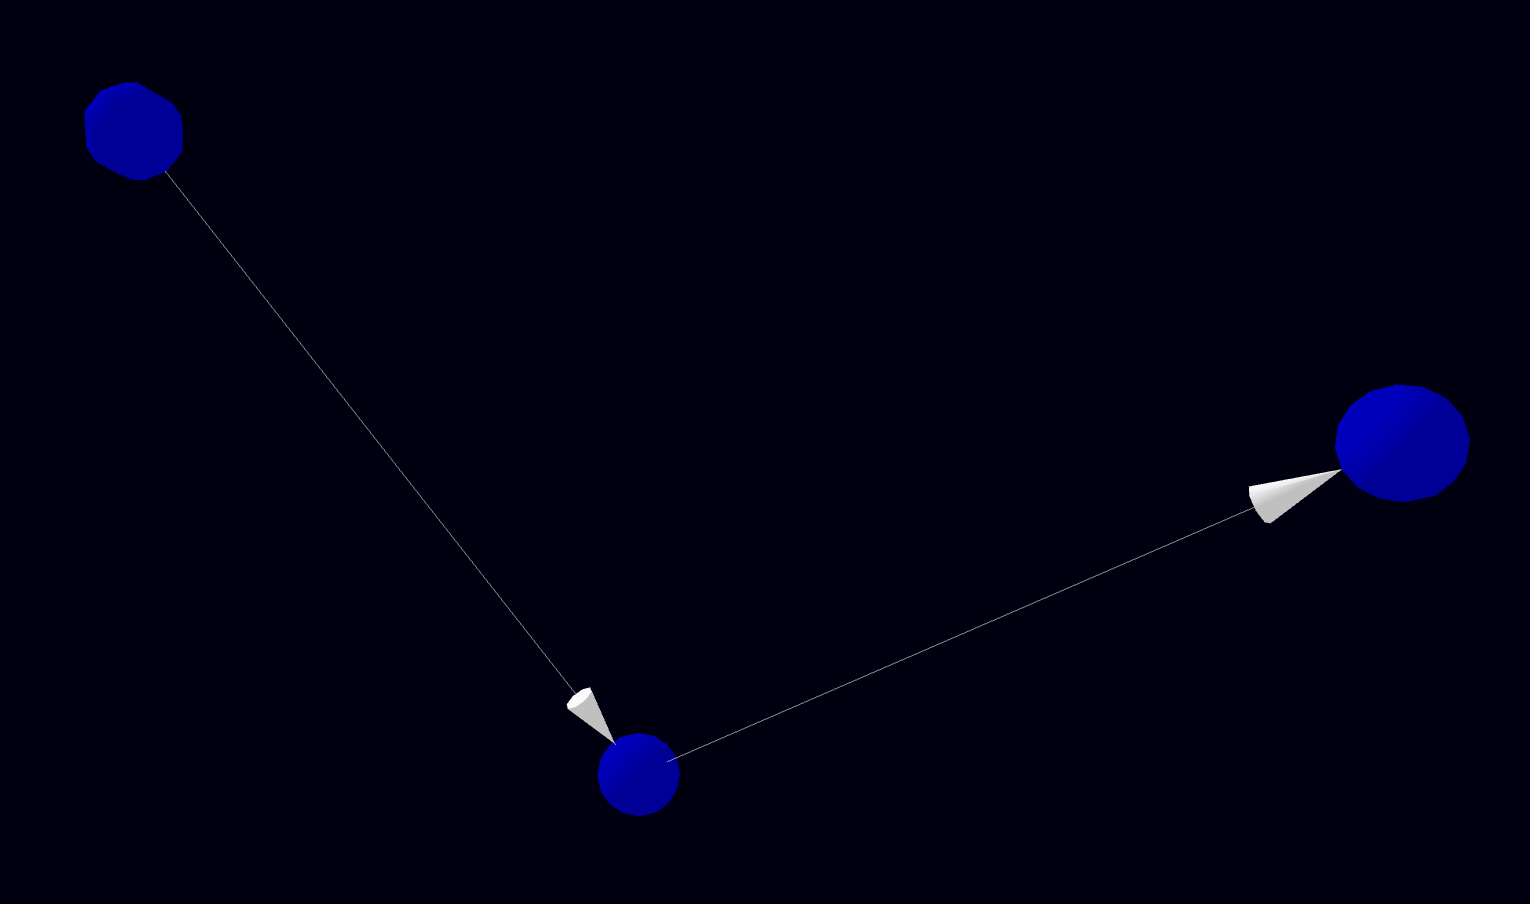
\includegraphics[width=\textwidth]{images/g1-graph.png}
        \caption{The $G_1$ subcategory}
        \label{fig:g1-graph}
    \end{subfigure}
    \hfill
    \begin{subfigure}[b]{0.48\textwidth}
        \centering
        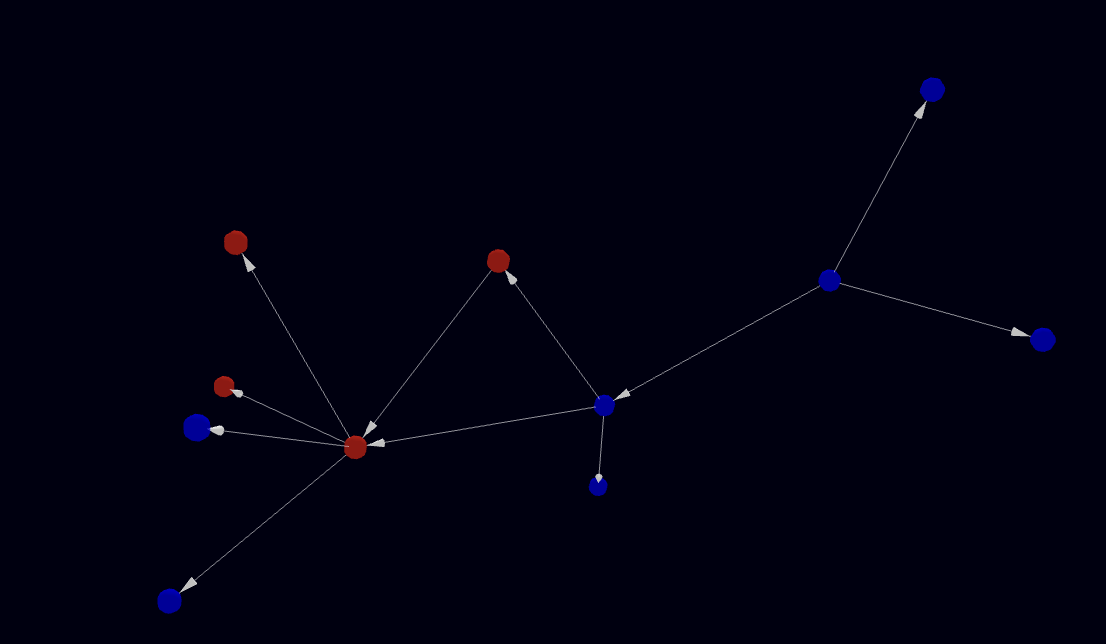
\includegraphics[width=\textwidth]{images/g2-graph.png}
        \caption{The $G_2$ subcategory}
        \label{fig:g2-graph}
    \end{subfigure}

    \vspace{1.5em} % Adds vertical space between the rows

    % Second row
    \begin{subfigure}[b]{0.48\textwidth}
        \centering
        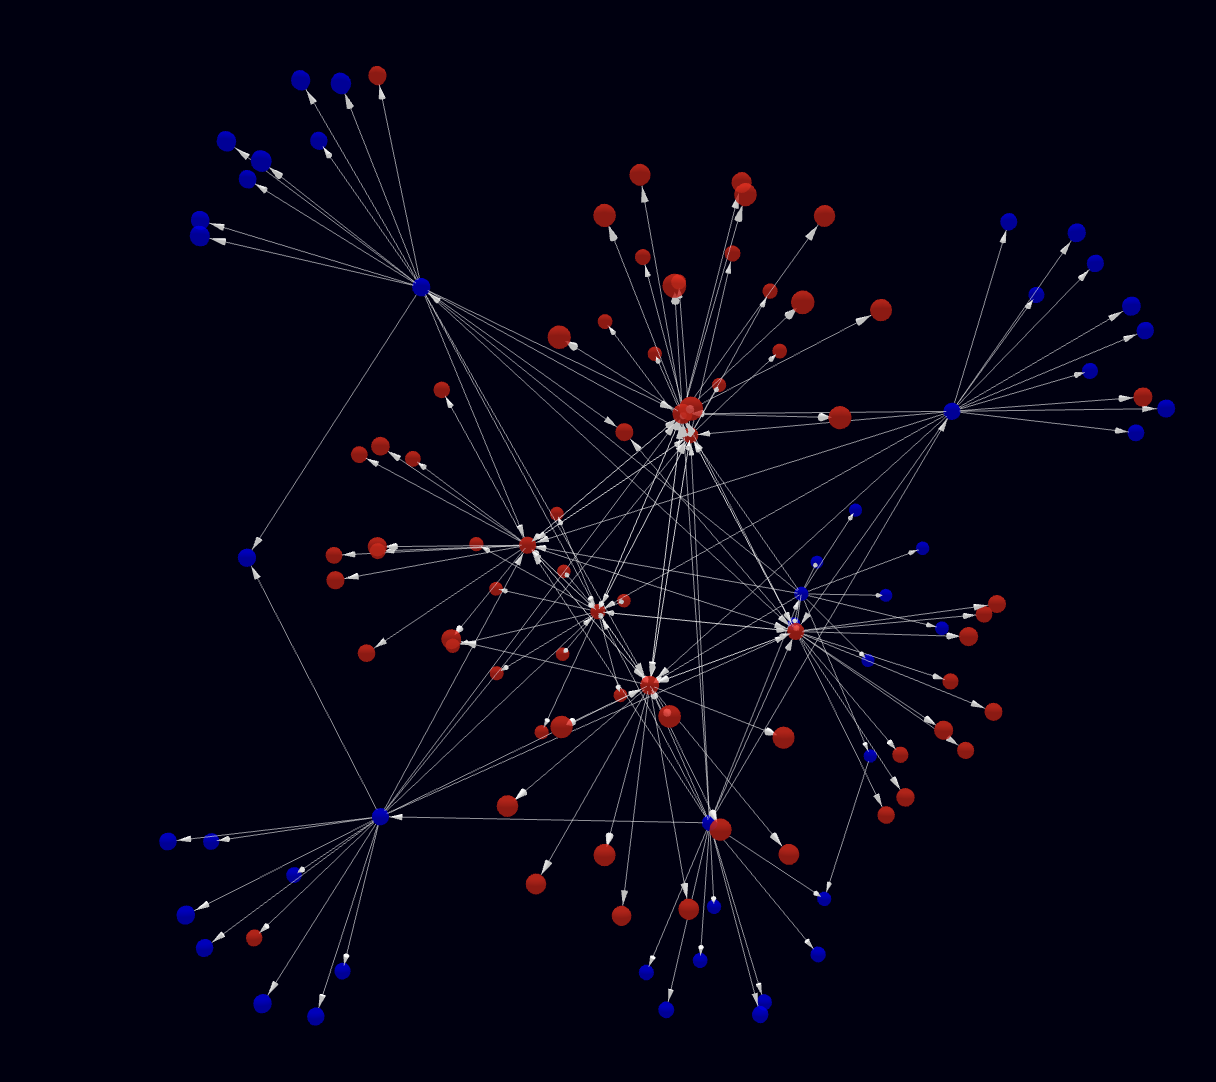
\includegraphics[width=\textwidth]{images/g3-graph.png}
        \caption{The $G_3$ subcategory}
        \label{fig:g3-graph}
    \end{subfigure}
    \hfill
    \begin{subfigure}[b]{0.48\textwidth}
        \centering
        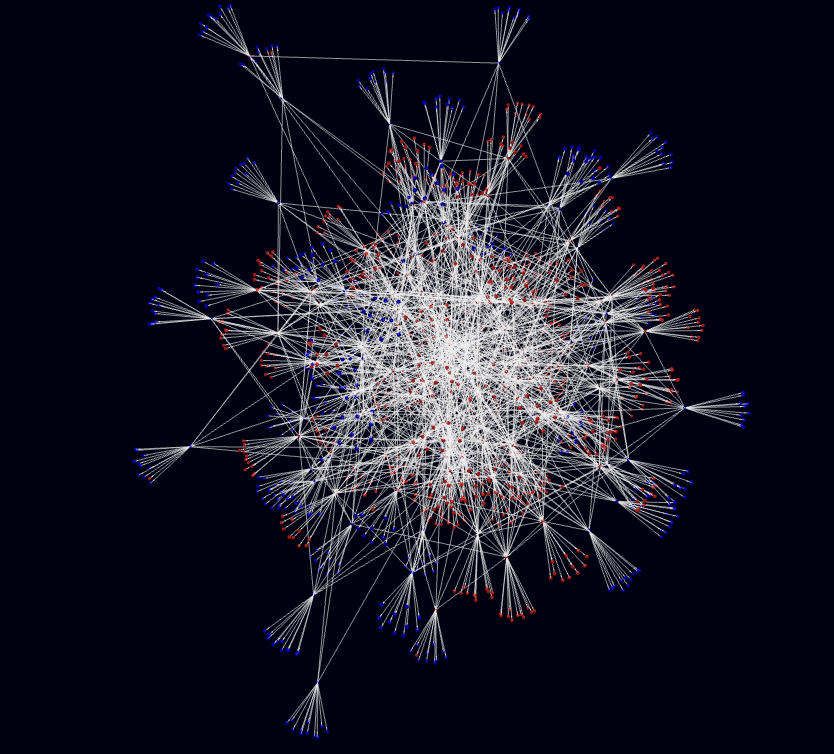
\includegraphics[width=\textwidth]{images/g4-graph.png}
        \caption{The $G_4$ subcategory}
        \label{fig:g4-graph}
    \end{subfigure}

    \caption{
        Overview of the $G_1$ through $G_4$ subcategories.
        Nodes represent propositions. They are blue if they have no witness or proof, and they are red if they have one.
        Edges are implications between propositions, i.e., there is an edge between nodes $P$ and $Q$ if there is a proof of $P \to Q$. 
    }
    \label{fig:g-grid}
\end{figure}